\documentclass[]{article}

% Imported Packages
%------------------------------------------------------------------------------
\usepackage{amssymb}
\usepackage{amstext}
\usepackage{amsthm}
\usepackage{amsmath}
\usepackage{enumerate}
\usepackage{fancyhdr}
\usepackage[margin=1in]{geometry}
\usepackage{graphicx}
\usepackage{setspace}
%------------------------------------------------------------------------------

% Header and Footer
%------------------------------------------------------------------------------
\pagestyle{plain}  
\renewcommand\headrulewidth{0.4pt}                                      
\renewcommand\footrulewidth{0.4pt}                                    
%------------------------------------------------------------------------------

% Title Details
%------------------------------------------------------------------------------
\title{Deliverable \#2}
\author{SE 3A04: Software Design II -- Large System Design}
\date{}                               
%------------------------------------------------------------------------------

% Document
%------------------------------------------------------------------------------
\begin{document}

\maketitle	

\section{Introduction}
\label{sec:introduction}
% Begin Section

This section of the High-Level Architectural Design provides an overview of everything included in the High-Level Architectural Design. 

\subsection{Purpose}
\label{sub:purpose}
% Begin SubSection
The purpose of this document is to provide a representation of the structure of the data and program components that will be required to build the ‘Movie Matcher’ software. This document will primarily be utilized by the developers of the software application and will be reviewed by the teaching assistants. 
% End SubSection

\subsection{System Description}
\label{sub:system_description}
% Begin SubSection
‘Movie Matcher’ is a mobile software application that will provide a platform through which users can find the name of a movie after being given specific details the user knows about the movie. The application must also display information relevant to any movies matching the user’s criteria. If the user successfully finds the movie that they were searching for, they should be directed to all nearly theaters that are currently screening the movie. If the movie is no longer in theaters, the user should be provided with links to purchase the movie. 
The primary goal of this software is to help users identify movies based on movie attributes the user inputs into the system. The software cannot guarantee to always find the correct result, or any result whatsoever if none of the inputted attributes match the movies in the database. The software will attempt to locate nearby movie theaters based on its interaction with the pre-implemented GPS in the user’s mobile device. The software will also require a stable internet connection to function and perform searches. 
% End SubSection

\subsection{Overview}
\label{sub:overview}
% Begin SubSection
This document is divided into 5 separate sections. The first section is this introduction. The second section consists of the Use Case Diagram, which is a representation of a user’s interaction with the system. The Use Case Diagram will be accompanied with a text description. The third section contains the Analysis Class Diagram which is a static structure diagram that serves the purpose of describing the structure of the software, by showing the system’s subclasses, methods, attributes and the relationships between objects. The fourth section provides an overview of the overall architectural design of the software application. It will show the division of the system into subsystems with high cohesion and low coupling, thereby following good software engineering principles. 
The fifth and final section will display the Class Responsibility Collaboration (CRC) Cards. A CRC card will be provided for each identified class. By organizing the document into 5 distinct sections with clear diagrams for each section, the audience will find the document easy to read and understand
% End SubSection

% End Section

\section{Use Case Diagram}
\label{sec:use_case_diagram}
% Begin Section
\begin{enumerate}[a)]
	\item The use case for the client side of the application.\newline
	\includegraphics[scale=0.5]{UseCaseClient.png}
	\newpage
	\item The use case for the server side of the application.\newline
	\includegraphics[scale=0.5]{UseCaseServer.png}
\end{enumerate}
% End Section

\section{Analysis Class Diagram}
\label{sec:analysis_class_diagram}
% Begin Section
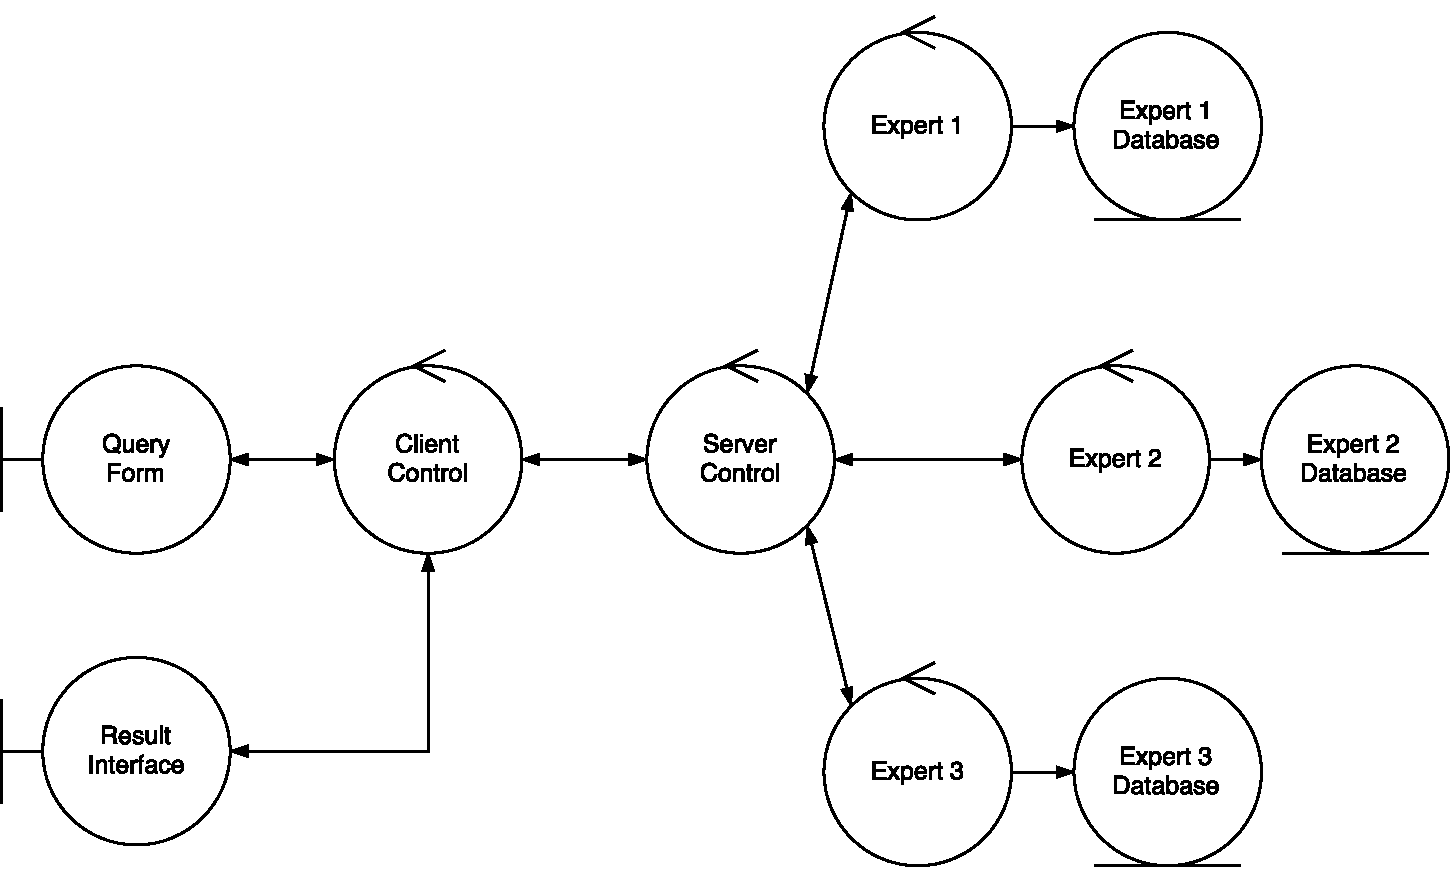
\includegraphics[width=\textwidth]{ACDRevised}
% End Section


\section{Architectural Design}
\label{sec:architectural_design}
% Begin Section\

\subsection{System Architecture}
\label{sub:system_architecture}
% Begin SubSection
The overall architecture of the system is a hybrid between a Client-Server Architecture and a Blackboard Architecture. Both of these architectures are needed to make the design more robust and simple.

In a Client-Server Architecture, there are many clients that communicate with a server. In the case of this system, this architecture makes sense because there is a client with a GUI that the users can use to make searches and have information displayed to them. There is also a server component that will contain large databases of information which would be too large to store in the client. The server can respond to a client's query by using the database of information. The reason why a Client-Server architecture is necessary is that the databases of movie information are very large and it would be too much to download considering that this system is a mobile application. This architecture allows the data to be stored on the server and only relevant parts are communicated to the client.

In the Blackboard Architecture there is a blackboard subsystem that stores data, and there is a knowledge source subsystem that stores domain specific data. In this system, the blackboard and knowledge subsystems are part of the server system. The blackboard is on the server and will contain the information about a movie, and what movie each expert thinks corresponds to this data. The knowledge source will be databases stored on the server because databases of movies are very large, much too large to store in the client system. The knowledge subsystem is the experts. The reason for using a Blackboard Architecture is that it allows for more experts to be easily added. It also makes it easy to combine the results from each individual expert in a centralized location.
% End SubSection

\subsection{Subsystems}
\label{sub:subsystems}
% Begin SubSection
\begin{description}
	\item[Blackboard] Provides information to the experts and combines the results.
	\item[Communication] Handles communication between client and server. Includes necessary encryption.
	\item[Knowledge] Contains many experts, each has a specific method of going from information about a movie, to what movie that information is about. Gets the information from the Blackboard subsystem and returns the result to it as well.
	\item[UI] Provides the user with a graphical user interface so they can interact with the client.
\end{description}
% End SubSection

% End Section
	
\section{Class Responsibility Collaboration (CRC) Cards}
\label{sec:class_responsibility_collaboration_crc_cards}
% Begin Section
This section should contain all of your CRC cards.

\begin{enumerate}[a)]
	\item Provide a CRC Card for each identified class
	\item Please use the format outlined in tutorial, i.e., 
	\begin{table}[ht]
		\centering
		\begin{tabular}{|p{5cm}|p{5cm}|}
		\hline 
		 \multicolumn{2}{|l|}{\textbf{Class Name: Client Query}} \\
		\hline
		\textbf{Responsibilities: } & \textbf{Collaborators:} \\
		\hline
		Decrypt the encrypted client query information and send it to server control.	
		\vspace{1in} & Server Control.\\
		
		\hline				
		\end{tabular}
	\end{table}
	
\begin{table}[ht]
		\centering
		\begin{tabular}{|p{5cm}|p{5cm}|}
		\hline 
		 \multicolumn{2}{|l|}{\textbf{Class Name: Server Query}} \\
		\hline
		\textbf{Responsibilities: } & \textbf{Collaborators:} \\
		\hline
		Format the decrypted client query to be used to query the experts.	
		\vspace{1in} & Server Control.\\
		
		\hline				
		\end{tabular}
	\end{table}

\begin{table}[ht]
		\centering
		\begin{tabular}{|p{5cm}|p{5cm}|}
		\hline 
		 \multicolumn{2}{|l|}{\textbf{Class Name: Client Results}} \\
		\hline
		\textbf{Responsibilities: } & \textbf{Collaborators:} \\
		\hline
		Retrieve the expert results and stores it.	
		\vspace{1in} & Server Control.\\
		
		\hline				
		\end{tabular}
	\end{table}

\begin{table}[ht]
		\centering
		\begin{tabular}{|p{5cm}|p{5cm}|}
		\hline 
		 \multicolumn{2}{|l|}{\textbf{Class Name: Client Interface}} \\
		\hline
		\textbf{Responsibilities: } & \textbf{Collaborators:} \\
		\hline
		Retrieve the server query. Use the server query to search the experts for information regarding the search query. Send the information retrieved from the expert search to the server control	
		\vspace{1in} & Server Control.\\
		
		\hline				
		\end{tabular}
	\end{table}

\begin{table}[ht]
		\centering
		\begin{tabular}{|p{5cm}|p{5cm}|}
		\hline 
		 \multicolumn{2}{|l|}{\textbf{Class Name: Server Control}} \\
		\hline
		\textbf{Responsibilities: } & \textbf{Collaborators:} \\
		\hline
		Handle client query, server query and expert results being sent and retrieved from other classes.	
		\vspace{1in} & Expert Interface, Expert Results, Server Query, Client Query.\\
		
		\hline				
		\end{tabular}
	\end{table}

\begin{table}[ht]
		\centering
		\begin{tabular}{|p{5cm}|p{5cm}|}
		\hline 
		 \multicolumn{2}{|l|}{\textbf{Class Name: Server Security Control}} \\
		\hline
		\textbf{Responsibilities: } & \textbf{Collaborators:} \\
		\hline
		Handle client query and query result being sent and retrieved from other classes.	
		\vspace{1in} & Server Control, Client Security Control.\\
		
		\hline				
		\end{tabular}
	\end{table}

\begin{table}[ht]
		\centering
		\begin{tabular}{|p{5cm}|p{5cm}|}
		\hline 
		 \multicolumn{2}{|l|}{\textbf{Class Name: Client Security Control}} \\
		\hline
		\textbf{Responsibilities: } & \textbf{Collaborators:} \\
		\hline
		Handle client query and query result being sent and retrieved from other classes.	
		\vspace{1in} & Server Security Control, Client Control.\\
		
		\hline				
		\end{tabular}
	\end{table}

\begin{table}[ht]
		\centering
		\begin{tabular}{|p{5cm}|p{5cm}|}
		\hline 
		 \multicolumn{2}{|l|}{\textbf{Class Name: Query Form}} \\
		\hline
		\textbf{Responsibilities: } & \textbf{Collaborators:} \\
		\hline
		Handle click events of selecting a search criterion. Handle click events of the search button. Send the query form information to client control.	
		\vspace{1in} & Client Control.\\
		
		\hline				
		\end{tabular}
	\end{table}


\begin{table}[ht]
		\centering
		\begin{tabular}{|p{5cm}|p{5cm}|}
		\hline 
		 \multicolumn{2}{|l|}{\textbf{Class Name: Client Query}} \\
		\hline
		\textbf{Responsibilities: } & \textbf{Collaborators:} \\
		\hline
		Encrypt the client query information and sends it to client control.
		\vspace{1in} & Client Control.\\
		
		\hline				
		\end{tabular}
	\end{table}

\begin{table}[ht]
		\centering
		\begin{tabular}{|p{5cm}|p{5cm}|}
		\hline 
		 \multicolumn{2}{|l|}{\textbf{Class Name: Client Control}} \\
		\hline
		\textbf{Responsibilities: } & \textbf{Collaborators:} \\
		\hline
		Handle client query information and client query results being passed from one class to another.	
		\vspace{1in} & Client Security Control.\\
		
		\hline				
		\end{tabular}
	\end{table}

\begin{table}[ht]
		\centering
		\begin{tabular}{|p{5cm}|p{5cm}|}
		\hline 
		 \multicolumn{2}{|l|}{\textbf{Class Name: Result Interface}} \\
		\hline
		\textbf{Responsibilities: } & \textbf{Collaborators:} \\
		\hline
		Retrieve the client query results. Display the client query results to the user.
		\vspace{1in} & Client Control.\\
		
		\hline				
		\end{tabular}
	\end{table}

\begin{table}[ht]
		\centering
		\begin{tabular}{|p{5cm}|p{5cm}|}
		\hline 
		 \multicolumn{2}{|l|}{\textbf{Class Name: Query Result}} \\
		\hline
		\textbf{Responsibilities: } & \textbf{Collaborators:} \\
		\hline
		Decrypt the encrypted client query results and sends it to client control.
		\vspace{1in} & Client Control.\\
		
		\hline				
		\end{tabular}
	\end{table}
\end{enumerate}
% End Section

\newpage
\clearpage
\appendix
\section{Division of Labour} \label{dlabour}
% Begin Section
\begin{tabular}{ |p{3cm}||p{2cm}|p{6cm}|p{1.5cm}|  }
 \hline
 \multicolumn{4}{|c|}{Contributions} \\
 \hline
 \textbf{Name}& \textbf{Student Number}& \textbf{Contribution}& \textbf{Signature}\\
 \hline
 Joshua &     &&   \\ 
 &&&   \\
 &&&   \\
 &&&   \\
 \hline
 Keyur  &    &  &\\
 &&&   \\
 &&&   \\
 &&&   \\
 \hline
 Justin &&& \\
 &&&   \\
 &&&   \\
 &&&   \\
 \hline
 Bilal & & & \\
 &&&   \\
 &&&   \\
 &&&   \\
 \hline
 Shaad &  & &\\
 &&&   \\
 &&&   \\
 &&&   \\
 \hline
 Abdullah & &  &\\
 &&&   \\
 &&&   \\
 &&&   \\
 \hline
\end{tabular}
% End Section

\end{document}
%------------------------------------------------------------------------------